
\begin{figure}
	\centering
	\subfloat[Number of GSS edges.]{
		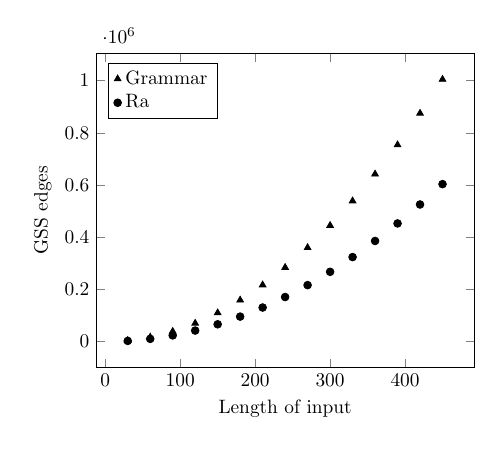
\begin{tikzpicture}[scale=.7]
		\begin{axis}[
		legend cell align=left,
		legend pos = north west,
		xlabel = {Length of input},
		ylabel = {GSS edges},
		%ymode=log
		]
		\addplot [only marks, mark=triangle*] coordinates {
			(30,4022) (60,17012) (90,39002) (120,69992) (150,109982) (180,158972) (210,216962) (240,283952) (270,359942) (300,444932) (330,538922) (360,641912) (390,753902) (420,874892) (450,1004882)
		};
		\addplot [only marks, mark=*] coordinates {
			(30,2452) (60,10282) (90,23512) (120,42142) (150,66172) (180,95602) (210,130432) (240,170662) (270,216292) (300,267322) (330,323752) (360,385582) (390,452812) (420,525442) (450,603472)
		};
		\legend{ 
			Grammar, 
			Ra
		};
		\end{axis}
		\end{tikzpicture}
		\label{fig:GSSedges}
	}
	~
	\subfloat[Time of parsing.]{
		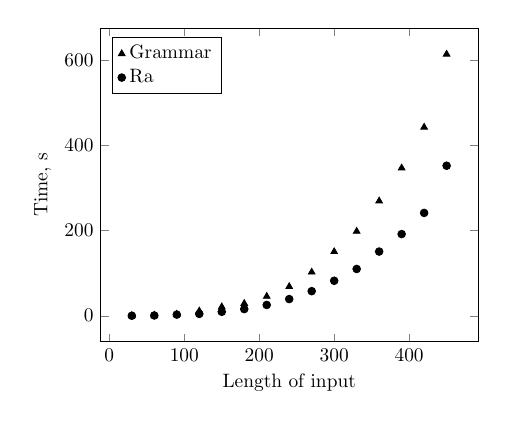
\begin{tikzpicture}[scale=.7]
		\begin{axis}[
		legend cell align=left,
		legend pos = north west,
		xlabel = {Length of input},
		ylabel = {Time, s},
		%ymode=log
		]
		\addplot [only marks, mark=triangle*] coordinates {
			(30,00.1690245) (60,01.1310924) (90,03.6899218) (120,11.1006359) (150,20.8163584) (180,28.7973458) (210,45.3640866) (240,68.3269546) (270,102.2953852) (300,150.2681210) (330,197.9508999) (360,269.1387530) (390,346.4999998) (420,442.0947044) (450,613.3386222)
		};
		\addplot [only marks, mark=*] coordinates {
			(30,00.0625041) (60,00.6562026) (90,02.6719009) (120,04.3594156) (150,09.2969549) (180,15.6406979) (210,25.3438039) (240,39.1251338) (270,57.6720586) (300,82.0470354) (330,109.7031754) (360,150.5466896) (390,191.5317906) (420,241.1571067) (450,351.8283519)
		};
		\legend{ 
			Grammar, 
			Ra
		};
		\end{axis}
		\end{tikzpicture}
		\label{fig:Time}
	}
	
	\subfloat[Number of SPPF nodes.]{
		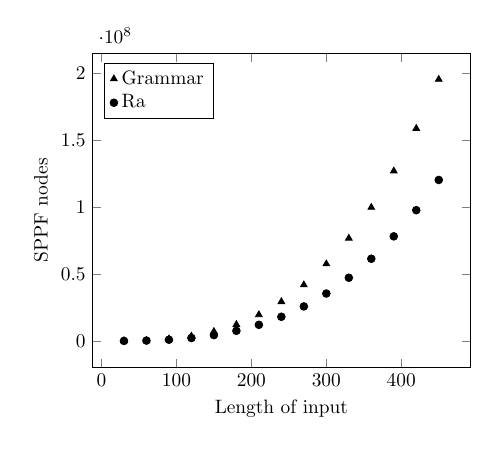
\begin{tikzpicture}[scale=.7]
		\begin{axis}[
		legend cell align=left,
		legend pos = north west,
		xlabel = {Length of input},
		ylabel = {SPPF nodes},
		%ymode=log
		]
		\addplot [only marks, mark=triangle*] coordinates {
			(30,49430) (60,429210) (90,1490290) (120,3583670) (150,7060350) (180,12271330) (210,19567610) (240,29300190) (270,41820070) (300,57478250) (330,76625730) (360,99613510) (390,126792590) (420,158513970) (450,195128650)
		};
		\addplot [only marks, mark=*] coordinates {
			(30,30695) (60,264835) (90,918375) (120,2207315) (150,4347655) (180,7555395) (210,12046535) (240,18037075) (270,25743015) (300,35380355) (330,47165095) (360,61313235) (390,78040775) (420,97563715) (450,120098055)
		};
		\legend{ 
			Grammar, 
			Ra
		};
		\end{axis}
		\end{tikzpicture}
		\label{fig:SPPFnodes}
	}
	~
	\subfloat[Memory usage]{
		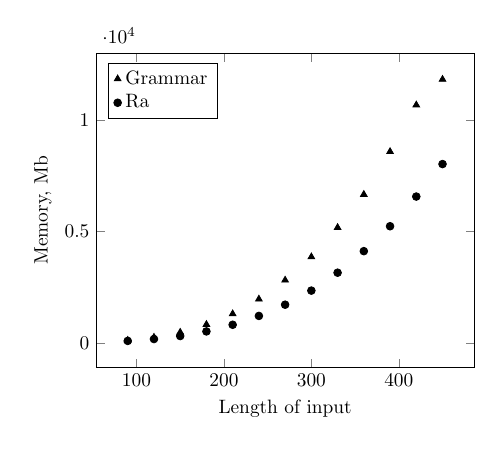
\begin{tikzpicture}[scale=.7]
		\begin{axis}[
		legend cell align=left,
		legend pos = north west,
		xlabel = {Length of input},
		ylabel = {Memory, Mb},
		%ymode=log
		]
		\addplot [only marks, mark=triangle*] coordinates {
			(90,130) (120,267) (150,491) (180,842) (210,1318) (240,1977) (270,2827) (300,3869) (330,5183) (360,6665) (390,8583) (420,10671) (450,11818)
		};
		\addplot [only marks, mark=*] coordinates {
			(90,106) (120,190) (150,325) (180,531) (210,829) (240,1225) (270,1728) (300,2359) (330,3161) (360,4126) (390,5242) (420,6571) (450,8026)
		};
		\legend{ 
			Grammar, 
			Ra
		};
		\end{axis}
		\end{tikzpicture}
		\label{fig:Memory}
	}
	
	\subfloat[Number of descriptors.]{
		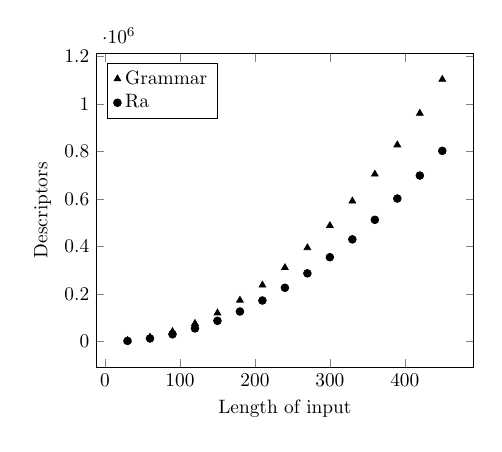
\begin{tikzpicture}[scale=.7]
		\begin{axis}[
		legend cell align=left,
		legend pos = north west,
		xlabel = {Length of input},
		ylabel = {Descriptors},
		%ymode=log
		]
		\addplot [only marks, mark=triangle*] coordinates {
			(30,4346) (60,18551) (90,42656) (120,76661) (150,120566) (180,174371) (210,238076) (240,311681) (270,395186) (300,488591) (330,591896) (360,705101) (390,828206) (420,961211) (450,1104116)
		};
		\addplot [only marks, mark=*] coordinates {
			(30,3181) (60,13531) (90,31081) (120,55831) (150,87781) (180,126931) (210,173281) (240,226831) (270,287581) (300,355531) (330,430681) (360,513031) (390,602581) (420,699331) (450,803281)
		};
		\legend{ 
			Grammar, 
			Ra
		};
		\end{axis}
		\end{tikzpicture}
		\label{fig:Descriptors}
	}
	\caption{Experiments results.}
	\label{expPlots}
\end{figure}